% LoRa-enabled remote patient monitoring - scientific report (IEEEtran conference format, max. 7 pages).
% Build: tectonic main.tex   |   latexmk -pdf main.tex   |   Overleaf (pdfLaTeX). See README.md.
\documentclass[conference]{IEEEtran}
\IEEEoverridecommandlockouts
\usepackage[T1]{fontenc}   % Times (ptm) in T1: same fonts under pdfLaTeX (Overleaf) and XeTeX (Tectonic)
\usepackage{cite}
\usepackage{amsmath,amssymb}
\usepackage{graphicx}
\usepackage{booktabs,tabularx,array,makecell}
\usepackage[caption=false,font=footnotesize]{subfig}
\usepackage{xcolor}
\usepackage{tikz}
\usetikzlibrary{positioning,arrows.meta,fit,backgrounds,calc,decorations.pathreplacing}
\usepackage{pgfplots}
\pgfplotsset{compat=1.18}
\usepgfplotslibrary{groupplots}
\usepackage{url}
\usepackage{microtype}
\usepackage[hidelinks]{hyperref}

\definecolor{hwc}{RGB}{190,95,20}    % hardware
\definecolor{swc}{RGB}{30,92,165}    % software
\definecolor{comc}{RGB}{24,128,72}   % radio / serial links
\definecolor{simc}{RGB}{105,105,105} % simulation
\newcolumntype{L}[1]{>{\raggedright\arraybackslash}p{#1}}
\newcolumntype{Y}{>{\raggedright\arraybackslash}X}
\graphicspath{{figures/}}
\newcommand{\ok}{\textcolor{comc}{\ensuremath{\checkmark}}}
\newcommand{\pend}{\textcolor{hwc}{pending}}

\begin{document}

\title{LoRa-Enabled Remote Patient Monitoring with Raspberry~Pi~5 Edge Processing, Network Simulation and Early-Warning Analytics}

\author{\IEEEauthorblockN{Iheb Bekir}
\IEEEauthorblockA{Industry~4.0 LoRa remote patient monitoring project}}

\maketitle

\begin{abstract}
Monitoring several ambulatory patients continuously requires a low-power radio link, trustworthy telemetry and timely interpretation, preferably without dependence on cellular or cloud infrastructure. This paper reports the design, implementation and evaluation status of a LoRa-based remote patient monitoring prototype. ESP32-S3 patient nodes encode heart rate, SpO$_2$, temperature and fall events into a 34-byte authenticated frame (HMAC-SHA256 tag, replay protection) carried over raw LoRa with application-level relays. Gateway software designed for a Raspberry~Pi~5 edge station validates and stores the frames, raises threshold and predictive alerts and serves a role-based web dashboard; a gradient-boosting early-warning model trained on synthetic data runs locally on the gateway. The multi-hop network was modelled in OMNeT++/INET/FLoRa with 20 patients and 3 relays. Results are reported by evidence category: 233 automated software tests pass; the simulation delivered 79 of 80 frames (98.75\,\%) with 78.1\,ms direct and up to 263.2\,ms three-hop delay; on held-out synthetic data the model reaches a PR-AUC of 0.543 at 1.6\,\% prevalence and flags 92 of 97 threshold-crossing episodes a median of 8.5\,min in advance, at 7.06 false-alarm episodes per patient-day. A bench LoRa link with a Heltec V3 receiver operates, and two Raspberry~Pi~5 UART integration faults were diagnosed and corrected; end-to-end physical validation with physiological sensors and deployment of the stack on the Pi remain pending. The system is a research prototype, not a medical device.
\end{abstract}

\begin{IEEEkeywords}
Remote patient monitoring, LoRa, edge computing, Raspberry Pi 5, OMNeT++/FLoRa, early-warning model.
\end{IEEEkeywords}

% =====================================================================================================================
\section{Introduction}
A ward, nursing home or village clinic may need to follow tens of patients whose vital signs change within minutes. Each observation is small (tens of bytes), but the link must be low-power, cover hundreds of metres through buildings, tolerate losses and remain \emph{trustworthy}: a forged or replayed vital-sign frame is a safety issue, not only a privacy one~\cite{islam2015iot}. LoRa chirp spread spectrum offers about $-124$\,dBm sensitivity at SF7/125\,kHz and kilometre-scale links at milliwatt power~\cite{augustin2016lora}, at the cost of kbit/s data rates, regulatory duty-cycle limits~\cite{etsi300220,adelantado2017limits} and collision-limited scalability~\cite{bor2016scale}; it has been shown viable for indoor health monitoring~\cite{petajajarvi2017health}.

Rather than LoRaWAN~\cite{lorawan104}, which presumes a network server, a join procedure and a star topology, the system uses raw LoRa with a custom authenticated frame and application-level relays, so that a single Raspberry~Pi~5 gateway can operate offline and keep patient data local. The contributions are: (i)~an end-to-end implementation (firmware, relay logic, gateway pipeline, role-based dashboard) built around a 34-byte authenticated frame; (ii)~a documented diagnosis of two Raspberry~Pi~5/Heltec~V3 UART integration faults; (iii)~an OMNeT++/INET/FLoRa model of a 20-patient multi-hop deployment, including the limits of its airtime model; (iv)~an on-gateway early-warning model evaluated at sample and episode level; and (v)~an evidence summary that keeps physical, software, simulation, analytical and model-evaluation results apart (Table~\ref{tab:evidence}).

% =====================================================================================================================
\section{System Architecture and Hardware}
\begin{figure*}[!t]
\centering
\resizebox{\textwidth}{!}{% Fig. 1 - system architecture and end-to-end data path (vector; edit here).
% Line styles: solid = implemented and covered by automated software tests; dashed = hardware validation pending;
% dotted = simulation. Colours: hardware (hwc), software (swc), radio/serial links (comc), simulation (simc).
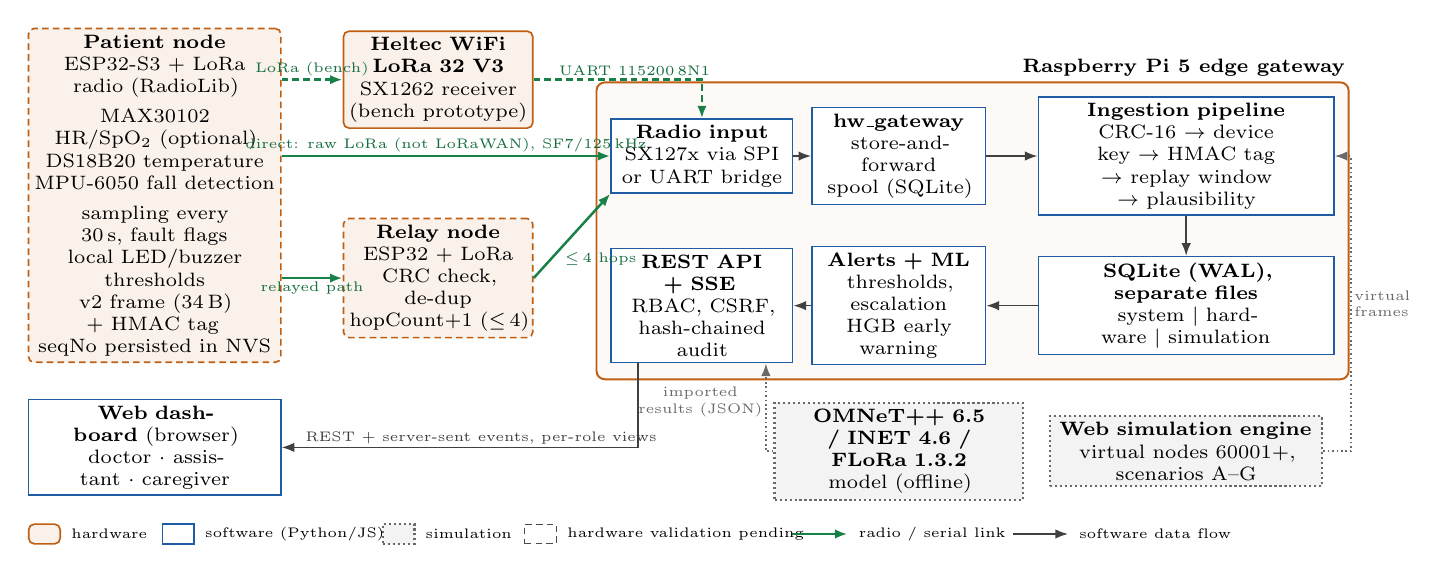
\begin{tikzpicture}[
  font=\scriptsize, >={Latex[length=1.6mm]},
  hw/.style={draw=hwc, fill=hwc!9, rounded corners=2pt, line width=.6pt, align=center, inner sep=2.2pt},
  sw/.style={draw=swc, fill=white, line width=.6pt, align=center, inner sep=2.2pt},
  simbox/.style={draw=simc, fill=simc!8, densely dotted, line width=.8pt, align=center, inner sep=2.2pt},
  pend/.style={dash pattern=on 2.4pt off 1.5pt},
  link/.style={->, line width=.9pt, draw=comc},
  flow/.style={->, line width=.6pt, draw=black!75},
  lbl/.style={font=\tiny, text=comc!85!black, align=center, inner sep=1pt},
]
% ---------------------------------------------------------------- patient side
\node[hw, pend, text width=3.05cm, minimum height=3.75cm] (pn) at (1.6,0.25) {%
  \textbf{Patient node}\\ ESP32-S3 + LoRa radio (RadioLib)\\[3pt]
  MAX30102 HR/SpO$_2$ (optional)\\ DS18B20 temperature\\ MPU-6050 fall detection\\[3pt]
  sampling every 30\,s, fault flags\\ local LED/buzzer thresholds\\ v2 frame (34\,B) + HMAC tag\\ seqNo persisted in NVS};
% ---------------------------------------------------------------- relay and bench receiver
\node[hw, pend, text width=2.25cm] (rl) at (5.2,-0.8) {\textbf{Relay node}\\ ESP32 + LoRa\\ CRC check, de-dup\\ hopCount${+}1$ ($\le$\,4)};
\node[hw, text width=2.25cm] (hb) at (5.2,1.72) {\textbf{Heltec WiFi LoRa 32 V3}\\ SX1262 receiver\\ (bench prototype)};
% ---------------------------------------------------------------- Raspberry Pi 5 gateway
\node[sw, text width=2.15cm] (g1) at (8.55,0.75) {\textbf{Radio input}\\ SX127x via SPI\\ or UART bridge};
\node[sw, text width=2.05cm] (g2) at (11.05,0.75) {\textbf{hw\_gateway}\\ store-and-forward\\ spool (SQLite)};
\node[sw, text width=3.6cm]  (g3) at (14.7,0.75) {\textbf{Ingestion pipeline}\\ CRC-16 $\to$ device key $\to$ HMAC tag\\ $\to$ replay window $\to$ plausibility};
\node[sw, text width=3.6cm]  (g4) at (14.7,-1.15) {\textbf{SQLite (WAL), separate files}\\ system $|$ hardware $|$ simulation};
\node[sw, text width=2.05cm] (g5) at (11.05,-1.15) {\textbf{Alerts + ML}\\ thresholds, escalation\\ HGB early warning};
\node[sw, text width=2.15cm] (g6) at (8.55,-1.15) {\textbf{REST API + SSE}\\ RBAC, CSRF,\\ hash-chained audit};
\begin{scope}[on background layer]
  \node[draw=hwc, fill=hwc!4, rounded corners=3pt, line width=.7pt, fit=(g1)(g2)(g3)(g4)(g5)(g6), inner sep=5pt,
        label={[font=\scriptsize\bfseries, anchor=south east, inner sep=1.5pt]north east:Raspberry Pi 5 edge gateway}] (gw) {};
\end{scope}
% ---------------------------------------------------------------- users and simulation sources
\node[sw, text width=3.05cm] (ui) at (1.6,-2.95) {\textbf{Web dashboard} (browser)\\ doctor $\cdot$ assistant $\cdot$ caregiver};
\node[simbox, text width=3.0cm] (om) at (11.05,-3.0) {\textbf{OMNeT++ 6.5 / INET 4.6 /}\\ \textbf{FLoRa 1.3.2} model (offline)};
\node[simbox, text width=3.3cm] (ws) at (14.7,-3.0) {\textbf{Web simulation engine}\\ virtual nodes 60001+, scenarios A--G};
% ---------------------------------------------------------------- radio / serial links
\draw[link] (pn.east |- g1.west) -- node[lbl, above, pos=0.5]{direct: raw LoRa (not LoRaWAN), SF7/125\,kHz} (g1.west);
\draw[link] (pn.east |- rl.west) -- node[lbl, below]{relayed path} (rl.west);
\draw[link] (rl.east) -- node[lbl, below right, pos=0.35]{$\le$\,4 hops} (g1.south west);
\draw[link, pend] (pn.east |- hb.west) -- node[lbl, above]{LoRa (bench)} (hb.west);
\draw[link, pend] (hb.east) -| node[lbl, pos=0.3, above]{UART 115200\,8N1} (g1.north);
% ---------------------------------------------------------------- software data path
\draw[flow] (g1) -- (g2);
\draw[flow] (g2) -- (g3);
\draw[flow] (g3) -- (g4);
\draw[flow] (g4) -- (g5);
\draw[flow] (g5) -- (g6);
\draw[flow] ($(g6.south west)+(0.35,0)$) |- node[lbl, pos=0.72, above, text=black!75]{REST + server-sent events, per-role views} (ui.east);
\draw[flow, simc, densely dotted] (om.west) -| node[lbl, pos=0.78, left, text=simc]{imported\\ results (JSON)} ($(g6.south east)+(-0.35,0)$);
\draw[flow, simc, densely dotted] (ws.east) -- ++(0.35,0) |- node[lbl, pos=0.25, right, text=simc, align=left]{virtual\\ frames} (g3.east);
% ---------------------------------------------------------------- legend
\begin{scope}[shift={(0.0,-4.05)}]
  \tikzset{key/.style={minimum width=4mm, minimum height=2.5mm, inner sep=0pt, anchor=center}, txt/.style={font=\tiny, anchor=west, inner sep=1pt}}
  \node[hw, key] at (0.2,0) {};               \node[txt] at (0.5,0) {hardware};
  \node[sw, key] at (1.9,0) {};               \node[txt] at (2.2,0) {software (Python/JS)};
  \node[simbox, key] at (4.7,0) {};           \node[txt] at (5.0,0) {simulation};
  \node[draw=black!70, pend, key] at (6.5,0) {}; \node[txt] at (6.8,0) {hardware validation pending};
  \draw[link] (9.7,0) -- (10.4,0);            \node[txt] at (10.5,0) {radio / serial link};
  \draw[flow] (12.5,0) -- (13.2,0);           \node[txt] at (13.3,0) {software data flow};
\end{scope}
\end{tikzpicture}
}
\caption{System architecture and end-to-end data path. Patient nodes transmit directly or through relays; the Raspberry~Pi~5 is designed to host the complete software stack (Python~3, Flask/waitress, SQLite, scikit-learn), so far executed and tested on an x86-64 PC. Physical, simulated (web engine) and offline OMNeT++ data follow separate paths and stores. Dashed outlines: hardware validation pending.}
\label{fig:architecture}
\end{figure*}

Fig.~\ref{fig:architecture} shows the three tiers. \emph{Patient nodes} sample every 30\,s, drive a local LED/buzzer from engineering thresholds and transmit either directly or, when out of range, through up to four relays. The \emph{gateway} receives frames from an SPI-attached SX127x transceiver (driver in the repository) or, on the bench, from a Heltec~V3 receiver over UART; a store-and-forward spool decouples reception from the platform API. The ingestion pipeline checks the CRC, resolves the device key, verifies the HMAC tag, applies a 62-frame replay window and plausibility limits (HR 20--250\,bpm, SpO$_2$ 50--100\,\%, temperature 25--45\,\textdegree C) and writes to one of three SQLite files: \emph{system} (users, audit), \emph{hardware} or \emph{simulation}. Physical and simulated data therefore never share a table, and virtual devices use identifiers $\geq$\,60001. Threshold, fall, sensor-fault, connectivity and predictive alerts reach browsers through server-sent events.

\begin{table*}[!t]
\caption{Hardware components: role, specifications relevant to the design, selection rationale and validation status}
\label{tab:hardware}
\centering\footnotesize
\begin{tabularx}{\textwidth}{@{}L{2.55cm}L{2.7cm}L{4.15cm}YL{2.45cm}@{}}
\toprule
Component & Role & Relevant specifications & Why selected & Status\\
\midrule
ESP32-S3~\cite{esp32s3} & patient/relay MCU & dual-core LX7 up to 240\,MHz, 512\,KB SRAM, SHA/AES accelerators, deep sleep & HMAC-SHA256 per frame and sensor handling with ample margin; mature Arduino/RadioLib~\cite{radiolib} toolchain & firmware written; protocol host-tested; not flashed\\
SX1276/78 or SX1262~\cite{sx1262} & raw LoRa PHY & SF7--12, 125\,kHz, up to +20/+22\,dBm, $-124$\,dBm at SF7/125\,kHz & licence-free long range without infrastructure; chip and band chosen explicitly at compile time (no default) & \pend\\
Heltec WiFi LoRa 32 V3~\cite{heltecv3} & bench receiver, UART bridge & ESP32-S3 + SX1262 + 0.96\,in OLED; CP2102 USB-UART on GPIO43/44 & integrated radio and display (counter, RSSI, SNR) speed up link debugging & operating (Fig.~\ref{fig:hardware_real})\\
MAX30102~\cite{max30102} & HR, SpO$_2$ & reflective PPG (red/IR), I$^2$C & single-chip HR/SpO$_2$ front-end & optional, disabled by default\\
DS18B20~\cite{ds18b20} & temperature & 1-Wire, $\pm$0.5\,\textdegree C ($-10$ to +85\,\textdegree C) & calibrated digital output, one GPIO & \pend\\
MPU-6050~\cite{mpu6050} & fall detection & 3-axis accelerometer + gyroscope, I$^2$C & free-fall ($<$\,0.5\,g) then impact ($>$\,2.5\,g) heuristic & \pend\\
Raspberry Pi 5~\cite{rpidocs} & edge gateway & 4$\times$ Cortex-A76 at 2.4\,GHz; 40-pin header with UART0 and SPI0 & runs ingestion, storage, inference and web server locally and offline & UART configured; stack runs on x86-64, Pi deployment \pend\\
\bottomrule
\end{tabularx}
\end{table*}

Table~\ref{tab:hardware} justifies each component. Hardware SHA acceleration makes per-frame authentication cheap compared with the radio. A Raspberry~Pi~5 rather than a microcontroller gateway is needed because the gateway runs a database, a web server and a tree-ensemble model concurrently; its header provides both the bench UART and the SPI bus of the SX127x driver.

\begin{figure}[!t]
\centering
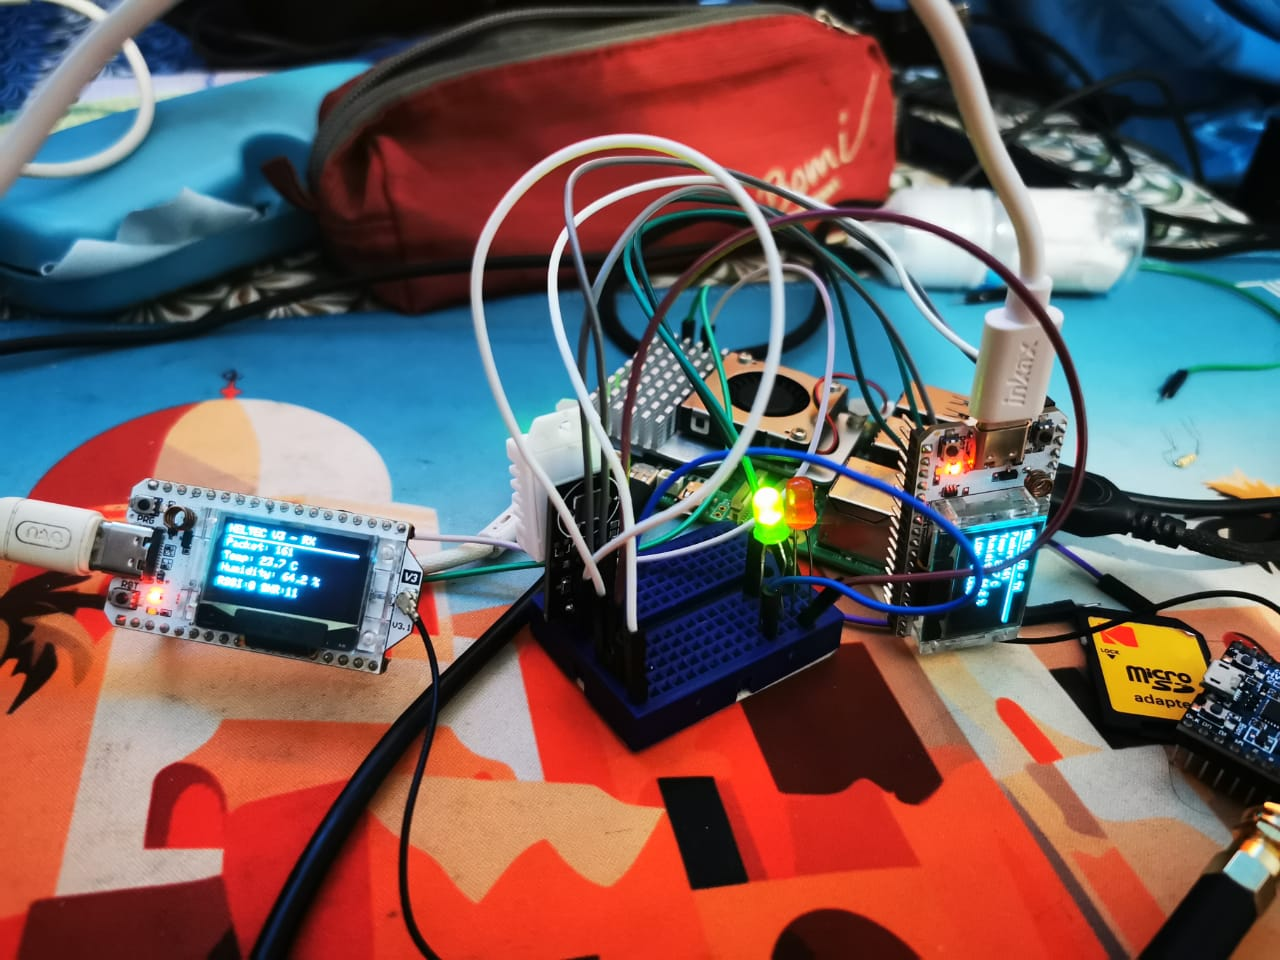
\includegraphics[width=\linewidth, trim=0 150 0 140, clip]{hardware_architecture_real.jpg}
\caption{Physical bench implementation. Left: Heltec WiFi LoRa 32 V3 operating as LoRa receiver; its OLED shows the received-packet counter (161), temperature (23.7\,\textdegree C), relative humidity (64.2\,\%), RSSI and SNR. Centre: breadboard with a DHT-type temperature/humidity sensor and status LEDs, in front of the Raspberry~Pi~5 (active cooler). Right: additional ESP32 board with OLED.}
\label{fig:hardware_real}
\end{figure}

\emph{Physical prototype.} Fig.~\ref{fig:hardware_real} shows the bench setup. The receiver's display evidences an operating point-to-point LoRa link carrying temperature/humidity readings. This bench firmware is not part of the repository and does not yet use the v2 physiological frame; the physiological sensor chain is implemented in firmware but not assembled. All physiological values in this paper are therefore synthetic or simulated.

% =====================================================================================================================
\section{Embedded Software and LoRa Communication}
\subsection{Firmware and frame format}
The patient firmware reads the sensors, classifies faults (a missing sensor sets a fault flag instead of sending zero) and encodes the v2 frame of Fig.~\ref{fig:frame}. The 32-bit sequence number is reserved in non-volatile storage in blocks of 32, surviving reboots with limited flash wear; a fall or critical event triggers an immediate frame, repeated twice with the same seqNo, with a 2\,s minimum transmission gap. Relays verify the CRC, suppress duplicates, enforce maxHopCount, increment hopCount and recompute the CRC. Because hopCount is excluded from the HMAC~\cite{rfc2104} input, relays need no key and cannot alter any other field undetected. The C++ encoder is cross-checked byte-for-byte against the Python reference by an automated test compiled with g++; the complete sketches have not been compiled for, or flashed onto, ESP32 hardware.

\begin{figure}[!t]
\centering
\resizebox{\linewidth}{!}{% Fig. 3 - protocol v2 frame layout (34 bytes, big-endian), from docs/PROTOCOL_SPECIFICATION.md.
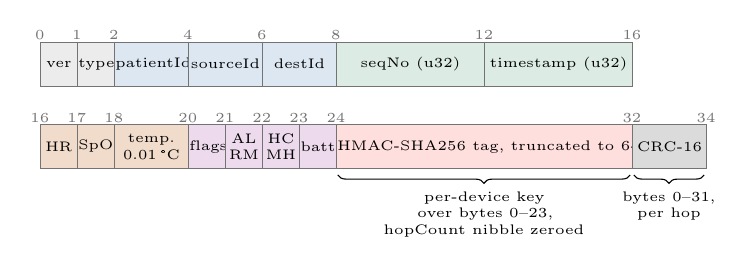
\begin{tikzpicture}[x=0.47cm, y=1cm, font=\tiny,
  fld/.style={draw=black!55, line width=.4pt, minimum height=0.56cm, inner sep=0.3pt, align=center, anchor=south west},
  off/.style={font=\tiny, text=black!55, anchor=south, inner sep=1pt}]
\newcommand{\fb}[5]{\node[fld, fill=#4, minimum width=#2*0.47cm] at (#1,#5) {#3};}
\newcommand{\of}[3]{\node[off] at (#1,#3+0.56) {#2};}
% row 1: bytes 0..15 (identity, routing, sequence, time)
\fb{0}{1}{ver}{gray!15}{0}   \of{0}{0}{0}
\fb{1}{1}{type}{gray!15}{0}  \of{1}{1}{0}
\fb{2}{2}{patientId}{swc!15}{0} \of{2}{2}{0}
\fb{4}{2}{sourceId}{swc!15}{0}  \of{4}{4}{0}
\fb{6}{2}{destId}{swc!15}{0}    \of{6}{6}{0}
\fb{8}{4}{seqNo (u32)}{comc!15}{0} \of{8}{8}{0}
\fb{12}{4}{timestamp (u32)}{comc!15}{0} \of{12}{12}{0} \of{16}{16}{0}
% row 2: bytes 16..33 (vital signs, status, authentication, integrity), drawn from x = 0
\fb{0}{1}{HR}{hwc!22}{-1.05}       \of{0}{16}{-1.05}
\fb{1}{1}{SpO$_2$}{hwc!22}{-1.05}  \of{1}{17}{-1.05}
\fb{2}{2}{temp.\\0.01\,\textdegree C}{hwc!22}{-1.05} \of{2}{18}{-1.05}
\fb{4}{1}{flags}{violet!14}{-1.05} \of{4}{20}{-1.05}
\fb{5}{1}{AL\\RM}{violet!14}{-1.05} \of{5}{21}{-1.05}
\fb{6}{1}{HC\\MH}{violet!14}{-1.05} \of{6}{22}{-1.05}
\fb{7}{1}{batt}{violet!14}{-1.05}  \of{7}{23}{-1.05}
\fb{8}{8}{HMAC-SHA256 tag, truncated to 64 bit}{red!13}{-1.05} \of{8}{24}{-1.05}
\fb{16}{2}{CRC-16}{gray!28}{-1.05} \of{16}{32}{-1.05} \of{18}{34}{-1.05}
\draw[decorate, decoration={brace, mirror, amplitude=3pt}, line width=.4pt] (8.05,-1.12) -- (15.95,-1.12)
  node[midway, below=2.5pt, align=center, text width=3.2cm] {per-device key over bytes 0--23,\\ hopCount nibble zeroed};
\draw[decorate, decoration={brace, mirror, amplitude=3pt}, line width=.4pt] (16.05,-1.12) -- (17.95,-1.12)
  node[midway, below=2.5pt, align=center] {bytes 0--31,\\ per hop};
\end{tikzpicture}
}
\caption{Protocol v2 frame (34\,B, big-endian; offsets above fields). AL/RM: alertLevel/routingMode nibbles; HC/MH: hopCount/maxHopCount. Version byte first, so legacy 16-B v1 frames remain distinguishable.}
\label{fig:frame}
\end{figure}

A binary encoding was chosen over JSON for airtime reasons: a compact JSON rendering of the same 15 measurement fields takes 241\,B (without tag or CRC), i.e.\ 379.1\,ms on air at SF7 versus 77.1\,ms for the v2 frame.

\subsection{Why raw LoRa, and at which cost}
LoRa suits patient nodes because traffic is sparse (one small frame per 30\,s) while range and battery life matter most; its limitations are airtime and contention. The time on air of an explicit-header frame with CRC is~\cite{semtech2013an1200}
\begin{align}
T_{\mathrm{oa}} &= \big(n_{\mathrm{pre}} + 4.25 + N_{\mathrm{s}}\big)\,\frac{2^{SF}}{BW}, \label{eq:toa}\\
N_{\mathrm{s}} &= 8 + \max\!\Big(\Big\lceil \tfrac{8PL - 4SF + 44}{4(SF - 2DE)} \Big\rceil (CR + 4),\, 0\Big), \nonumber
\end{align}
which gives 63 payload symbols and $T_{\mathrm{oa}} = 77.1$\,ms for $PL = 34$\,B, SF7, 125\,kHz, CR\,4/5 ($CR=1$), $DE=0$ and $n_{\mathrm{pre}}=8$. At one frame per 30\,s the duty cycle is 0.26\,\%, below the 1\,\% limit of common 868\,MHz SRD sub-bands~\cite{etsi300220}. Contention is the binding constraint: under a pure-ALOHA approximation without capture, $N=20$ nodes on one channel and SF yield an offered load $G = N T_{\mathrm{oa}}/T = 0.051$ and a frame success probability $e^{-2G} = 0.90$ (theoretical estimate), so scaling beyond a few tens of patients per channel requires several channels/SFs or scheduled transmissions. Table~\ref{tab:radio} lists the radio configuration of the firmware and of the simulation model.

\begin{table}[!t]
\caption{Radio and protocol parameters (repository configuration)}
\label{tab:radio}
\centering\footnotesize
\begin{tabularx}{\linewidth}{@{}L{1.85cm}YY@{}}
\toprule
Parameter & Firmware / Pi gateway & OMNeT++/FLoRa model\\
\midrule
Frequency & no default; must be set legally (e.g.\ 868.1\,MHz) & 868\,MHz\\
BW / SF / CR & 125\,kHz / SF7 / 4/5 & 125\,kHz / SF7 / \texttt{codeRate}\,=\,4\\
TX power & 14\,dBm & 14\,dBm\\
Sync word & 0x12 (private, not LoRaWAN) & --\\
Payload & 34\,B v2 frame & 70\,B chunk; airtime from fixed 20\,B\\
Interval / hops & 30\,s / $\leq$\,4 & 30\,s / $\leq$\,4\\
Time on air & 77.1\,ms (Eq.~\ref{eq:toa}) & 78.08\,ms node, 61.70\,ms relay\\
Bench UART & 115200\,8N1, GPIO2$\to$GPIO15 & --\\
\bottomrule
\end{tabularx}
\end{table}

% =====================================================================================================================
\section{Raspberry Pi 5 Integration and UART Troubleshooting}
On the bench, the Heltec~V3 receives LoRa packets and forwards them to the Raspberry~Pi~5 over a one-way UART (Fig.~\ref{fig:uart}). Reading \texttt{/dev/serial0} returned no data. The investigation isolated two independent configuration faults.

\emph{Pi~5 UART routing.} On the Pi~5, \texttt{/dev/serial0} pointed to \texttt{/dev/ttyAMA10}, the debug UART on the dedicated three-pin connector, while UART0 was not routed to GPIO14/15 of the 40-pin header~\cite{rpidocs}. Adding \texttt{dtoverlay=uart0-pi5} to \texttt{/boot/firmware/config.txt} and rebooting routes TXD0/RXD0 to GPIO14/15, which \texttt{pinctrl get 14-15} must then report; the header UART is \texttt{/dev/ttyAMA0}. The fault was therefore device selection and pin routing, not confirmed damage to a pin.

\emph{Heltec TX pin.} GPIO43/44 carry the ESP32-S3 UART0 that is wired to the on-board CP2102 USB bridge used for the serial console and flashing, so they cannot serve as an independent external UART. The ESP32-S3 GPIO matrix allows UART1 to be mapped to a free pin: \texttt{HardwareSerial PiSerial(1); PiSerial.begin(115200, SERIAL\_8N1, -1, 2);} uses UART1 with RX disabled ($-1$) and TX on GPIO2. Since the link is one-way, only Heltec TX$\to$Pi RX (GPIO15, pin~10) and ground (pin~6) are wired; both sides use 3.3\,V logic, so no level shifter is needed. Table~\ref{tab:uartcmd} lists the verification commands.

\begin{figure}[!t]
\centering
\resizebox{\linewidth}{!}{% Fig. 4 - bench UART wiring between the Heltec V3 receiver and the Raspberry Pi 5 (one direction only).
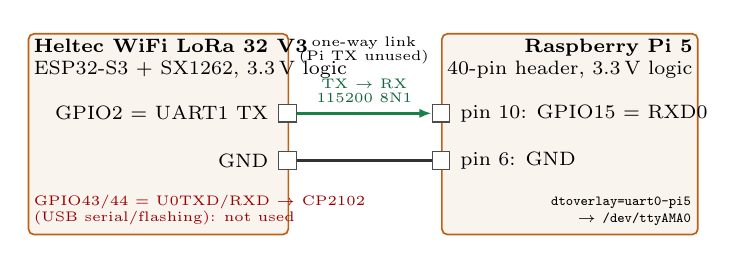
\begin{tikzpicture}[font=\scriptsize, >={Latex[length=1.6mm]},
  board/.style={draw=hwc, fill=hwc!7, rounded corners=2pt, line width=.6pt},
  pin/.style={draw=black!70, fill=white, minimum width=2.2mm, minimum height=2.2mm, inner sep=0pt}]
% Heltec V3
\node[board, minimum width=3.3cm, minimum height=2.55cm, anchor=south west] (h) at (0,0) {};
\node[anchor=north west, align=left, inner sep=2pt] at (h.north west) {\textbf{Heltec WiFi LoRa 32 V3}\\ ESP32-S3 + SX1262, 3.3\,V logic};
\node[pin] (htx) at (3.3,1.55) {}; \node[anchor=east, align=right] at (3.18,1.55) {GPIO2 = UART1 TX};
\node[pin] (hgnd) at (3.3,0.95) {}; \node[anchor=east] at (3.18,0.95) {GND};
\node[anchor=south west, align=left, font=\tiny, text=red!60!black, inner sep=2pt] at (0,0.05)
  {GPIO43/44 = U0TXD/RXD $\to$ CP2102\\ (USB serial/flashing): not used};
% Raspberry Pi 5 header
\node[board, minimum width=3.25cm, minimum height=2.55cm, anchor=south west] (p) at (5.25,0) {};
\node[anchor=north east, align=right, inner sep=2pt] at (p.north east) {\textbf{Raspberry Pi 5}\\ 40-pin header, 3.3\,V logic};
\node[pin] (prx) at (5.25,1.55) {}; \node[anchor=west] at (5.37,1.55) {pin 10: GPIO15 = RXD0};
\node[pin] (pgnd) at (5.25,0.95) {}; \node[anchor=west] at (5.37,0.95) {pin 6: GND};
\node[anchor=south east, align=right, font=\tiny, inner sep=2pt] at (8.5,0.05) {\texttt{dtoverlay=uart0-pi5}\\ $\to$ \texttt{/dev/ttyAMA0}};
% wires
\draw[->, line width=1.1pt, draw=comc] (htx) -- node[above, font=\tiny, text=comc!80!black, align=center] {TX $\to$ RX\\[-1pt] 115200 8N1} (prx);
\draw[line width=1.1pt, draw=black!80] (hgnd) -- (pgnd);
\node[font=\tiny, align=center] at (4.27,2.35) {one-way link\\[-1pt](Pi TX unused)};
\end{tikzpicture}
}
\caption{Bench UART wiring between the Heltec~V3 and the Raspberry~Pi~5 header. TX connects to RX; the Pi transmit line is not used.}
\label{fig:uart}
\end{figure}

\begin{table}[!t]
\caption{Raspberry Pi 5 UART verification commands}
\label{tab:uartcmd}
\centering\footnotesize
\begin{tabularx}{\linewidth}{@{}L{2.25cm}Y@{}}
\toprule
Purpose & Command\\
\midrule
Identify board & \texttt{cat /proc/device-tree/model}\\
Serial alias & \texttt{ls -l /dev/serial0}\\
Enable header UART0 & \texttt{dtoverlay=uart0-pi5} in \texttt{config.txt}, reboot\\
Pin functions & \texttt{pinctrl get 14-15} (TXD0, RXD0)\\
Configure port & \texttt{sudo stty -F /dev/ttyAMA0 115200 raw -echo}\\
Read data & \texttt{sudo cat /dev/ttyAMA0}\\
Port in use? & \texttt{sudo fuser -v /dev/ttyAMA0}\\
\bottomrule
\end{tabularx}
\end{table}

\emph{Status.} The configuration changes and wiring are established, but the available record does not conclusively show packets arriving on \texttt{/dev/ttyAMA0}; final UART validation is pending. The repository's gateway already accepts one hex-encoded frame per line on standard input, so a Heltec firmware that forwards raw v2 frames as hex lines would connect through \texttt{/dev/ttyAMA0} without new gateway code, and the HMAC would then protect the frame end-to-end across the UART hop.

% =====================================================================================================================
\section{OMNeT++/INET/FLoRa Network Simulation}
\subsection{Environment and purpose}
The bench validates interfaces, not network behaviour. OMNeT++~6.5.0~\cite{varga2008omnet} with INET~4.6.0~\cite{inet} and FLoRa~1.3.2~\cite{slabicki2018flora}, managed by \texttt{opp\_env} under WSL, allows controlled study of node count, gateway placement, relaying, path loss and collisions that cannot yet be tested physically. Table~\ref{tab:simcfg} shows what was configured and what was run.

\begin{table}[!t]
\caption{Simulation configurations and their status (ADR on: node and network server)}
\label{tab:simcfg}
\centering\footnotesize
\begin{tabularx}{\linewidth}{@{}L{2.2cm}L{0.8cm}cL{0.62cm}Y@{}}
\toprule
Configuration & Nodes & GW & ADR & Status\\
\midrule
n100-gw1 & 100 & 1 & on & started; vector file only, no scalars: not evaluated\\
n1000-gw1-ADR & 1000 & 1 & on & examined, not run\\
n1000-gw1-noADR & 1000 & 1 & off & examined, not run\\
n1000-gw2 & 1000 & 2 & off & examined, not run\\
DistributedRPM (this work) & 20 + 3 relays & 1 & -- & run (120\,s), evaluated\\
\bottomrule
\end{tabularx}
\end{table}

\subsection{RPM network model}
The project model \texttt{DistributedRPMNetwork} places the doctor gateway at the centre, 20 patients on rings of 25, 45 and 80\,m (8/8/4 nodes) and 3 relays on a 30\,m ring. Patients 1--16 transmit directly; patients 17--20 enter an ordered relay chain using unicast LoRa MAC addresses, and each relay checks identity, destination, duplicates, previous hop and hop limit before incrementing hopCount. Propagation follows FLoRa's log-normal shadowing ($d_0=40$\,m, $\gamma=2.08$, $\sigma=3.57$\,dB), giving a median range of about 129\,m at 14\,dBm for $-124$\,dBm sensitivity. Two FLoRa adaptations were needed (Table~\ref{tab:challenges}). The fixed SF7 suits the short distances; adaptive data rate (ADR)~\cite{slabicki2018flora} trades airtime against link margin, but it converges over many uplinks and may lag behind the body shadowing of mobile patients, so its benefit must be measured (n1000 ADR/no-ADR pair) rather than assumed.

\begin{figure}[!t]
\centering
\subfloat[Qtenv view of \texttt{DistributedRPMNetwork}: packet labels carry patient, sequence, vital signs and alert type.]{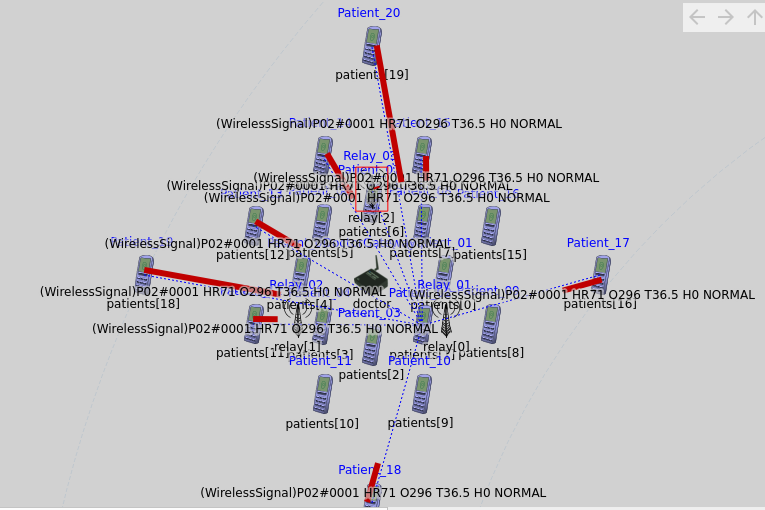
\includegraphics[width=0.9\linewidth]{omnet_flora_simulation.png}\label{fig:omnet_topo}}\\[-1pt]
\subfloat[\texttt{LoRaMedium} statistics printed by \texttt{finish()}.]{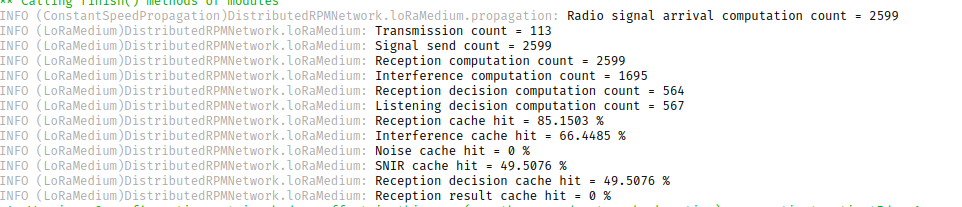
\includegraphics[width=0.97\linewidth]{omnet_flora_log.png}\label{fig:omnet_log}}
\caption{OMNeT++/FLoRa environment used to configure and investigate the multi-hop LoRa network (screenshots).}
\label{fig:omnet_flora}
\end{figure}

\subsection{Results and interpretation}
In the evaluated 120\,s run, 80 measurements were generated and 79 reached the doctor valid (PDR $=79/80=98.75$\,\%): 64 direct and 15 relay-assisted, with no invalid frames, no duplicates and no collisions. The doctor radio started 113 receptions, i.e.\ the 80 patient frames plus 33 relay forwards (7, 11 and 15 by relays 1--3), matching the transmission count in Fig.~\ref{fig:omnet_log}; 111 finished correctly. The single loss (patient~18, first frame) was traced to a reception at about $-124.8$\,dBm at relay~1, below sensitivity: a probabilistic shadowing outcome on the outer ring, not a protocol error. Fig.~\ref{fig:delay} shows the end-to-end delay, measured from frame creation at the patient to valid reception at the doctor.

\begin{figure}[!t]
\centering
% Fig. - OMNeT++/FLoRa end-to-end delay per hop count (data: figures/data/sim_delay_summary.dat,
% produced by tools/make_figure_data.py from the doctor.app vectors of run r6; n = 64, 4, 4, 7 packets).
\begin{tikzpicture}
\begin{axis}[
  width=\linewidth, height=3.5cm, ybar=1pt, bar width=8pt, ymin=0, ymax=400, ytick={0,100,200,300},
  xlabel={Relay hops traversed (hopCount)}, ylabel={Delay (ms)},
  xtick={0,1,2,3}, enlarge x limits=0.17, ymajorgrids, grid style={black!12},
  tick label style={font=\scriptsize}, label style={font=\scriptsize},
  legend style={font=\tiny, at={(0.01,0.98)}, anchor=north west, draw=none, fill=none, row sep=-1pt},
  legend cell align=left,
  nodes near coords, every node near coord/.append style={font=\tiny, rotate=90, anchor=west, /pgf/number format/fixed, /pgf/number format/precision=1},
]
\addplot[fill=swc!65, draw=swc] table[x=hop, y=sim_ms] {figures/data/sim_delay_summary.dat};
\addplot[fill=hwc!40, draw=hwc] table[x=hop, y=analytic34_ms] {figures/data/sim_delay_summary.dat};
\legend{{simulated (FLoRa airtime model)}, {analytical, 34-B v2 frame, Eq.~(\ref{eq:toa})}}
\end{axis}
\end{tikzpicture}

\caption{End-to-end delay per number of relay hops: OMNeT++/FLoRa run (blue; $n$ = 64, 4, 4 and 7 frames, identical delays within each group) versus analytical airtime of the real 34-B frame with immediate forwarding (orange).}
\label{fig:delay}
\end{figure}

The simulated delays are airtime-dominated and inherit a simplification of FLoRa~1.3.2: its transmitter computes airtime from a fixed payload of 20\,B for end nodes and 15\,B for gateway-type radios (coding term $\texttt{codeRate}+4$, integer division), hence exactly 78.08\,ms direct and $+$61.70\,ms per relay hop, independent of the actual frame. With the real 34-B frame each hop would add at least 77.1\,ms plus processing. Patients start 1.5\,s apart and then transmit strictly every 30\,s, so their frames never overlap, which explains the absence of collisions. Random-access contention (Section~III-B), terrain and mobility therefore remain to be studied, and simulation cannot replace on-site radio measurements.

% =====================================================================================================================
\section{Web Dashboard}
\begin{figure*}[!t]
\centering
\subfloat[Clinical overview (doctor): KPIs, sensor-to-response data-flow counters, live patient cards and active alerts.]{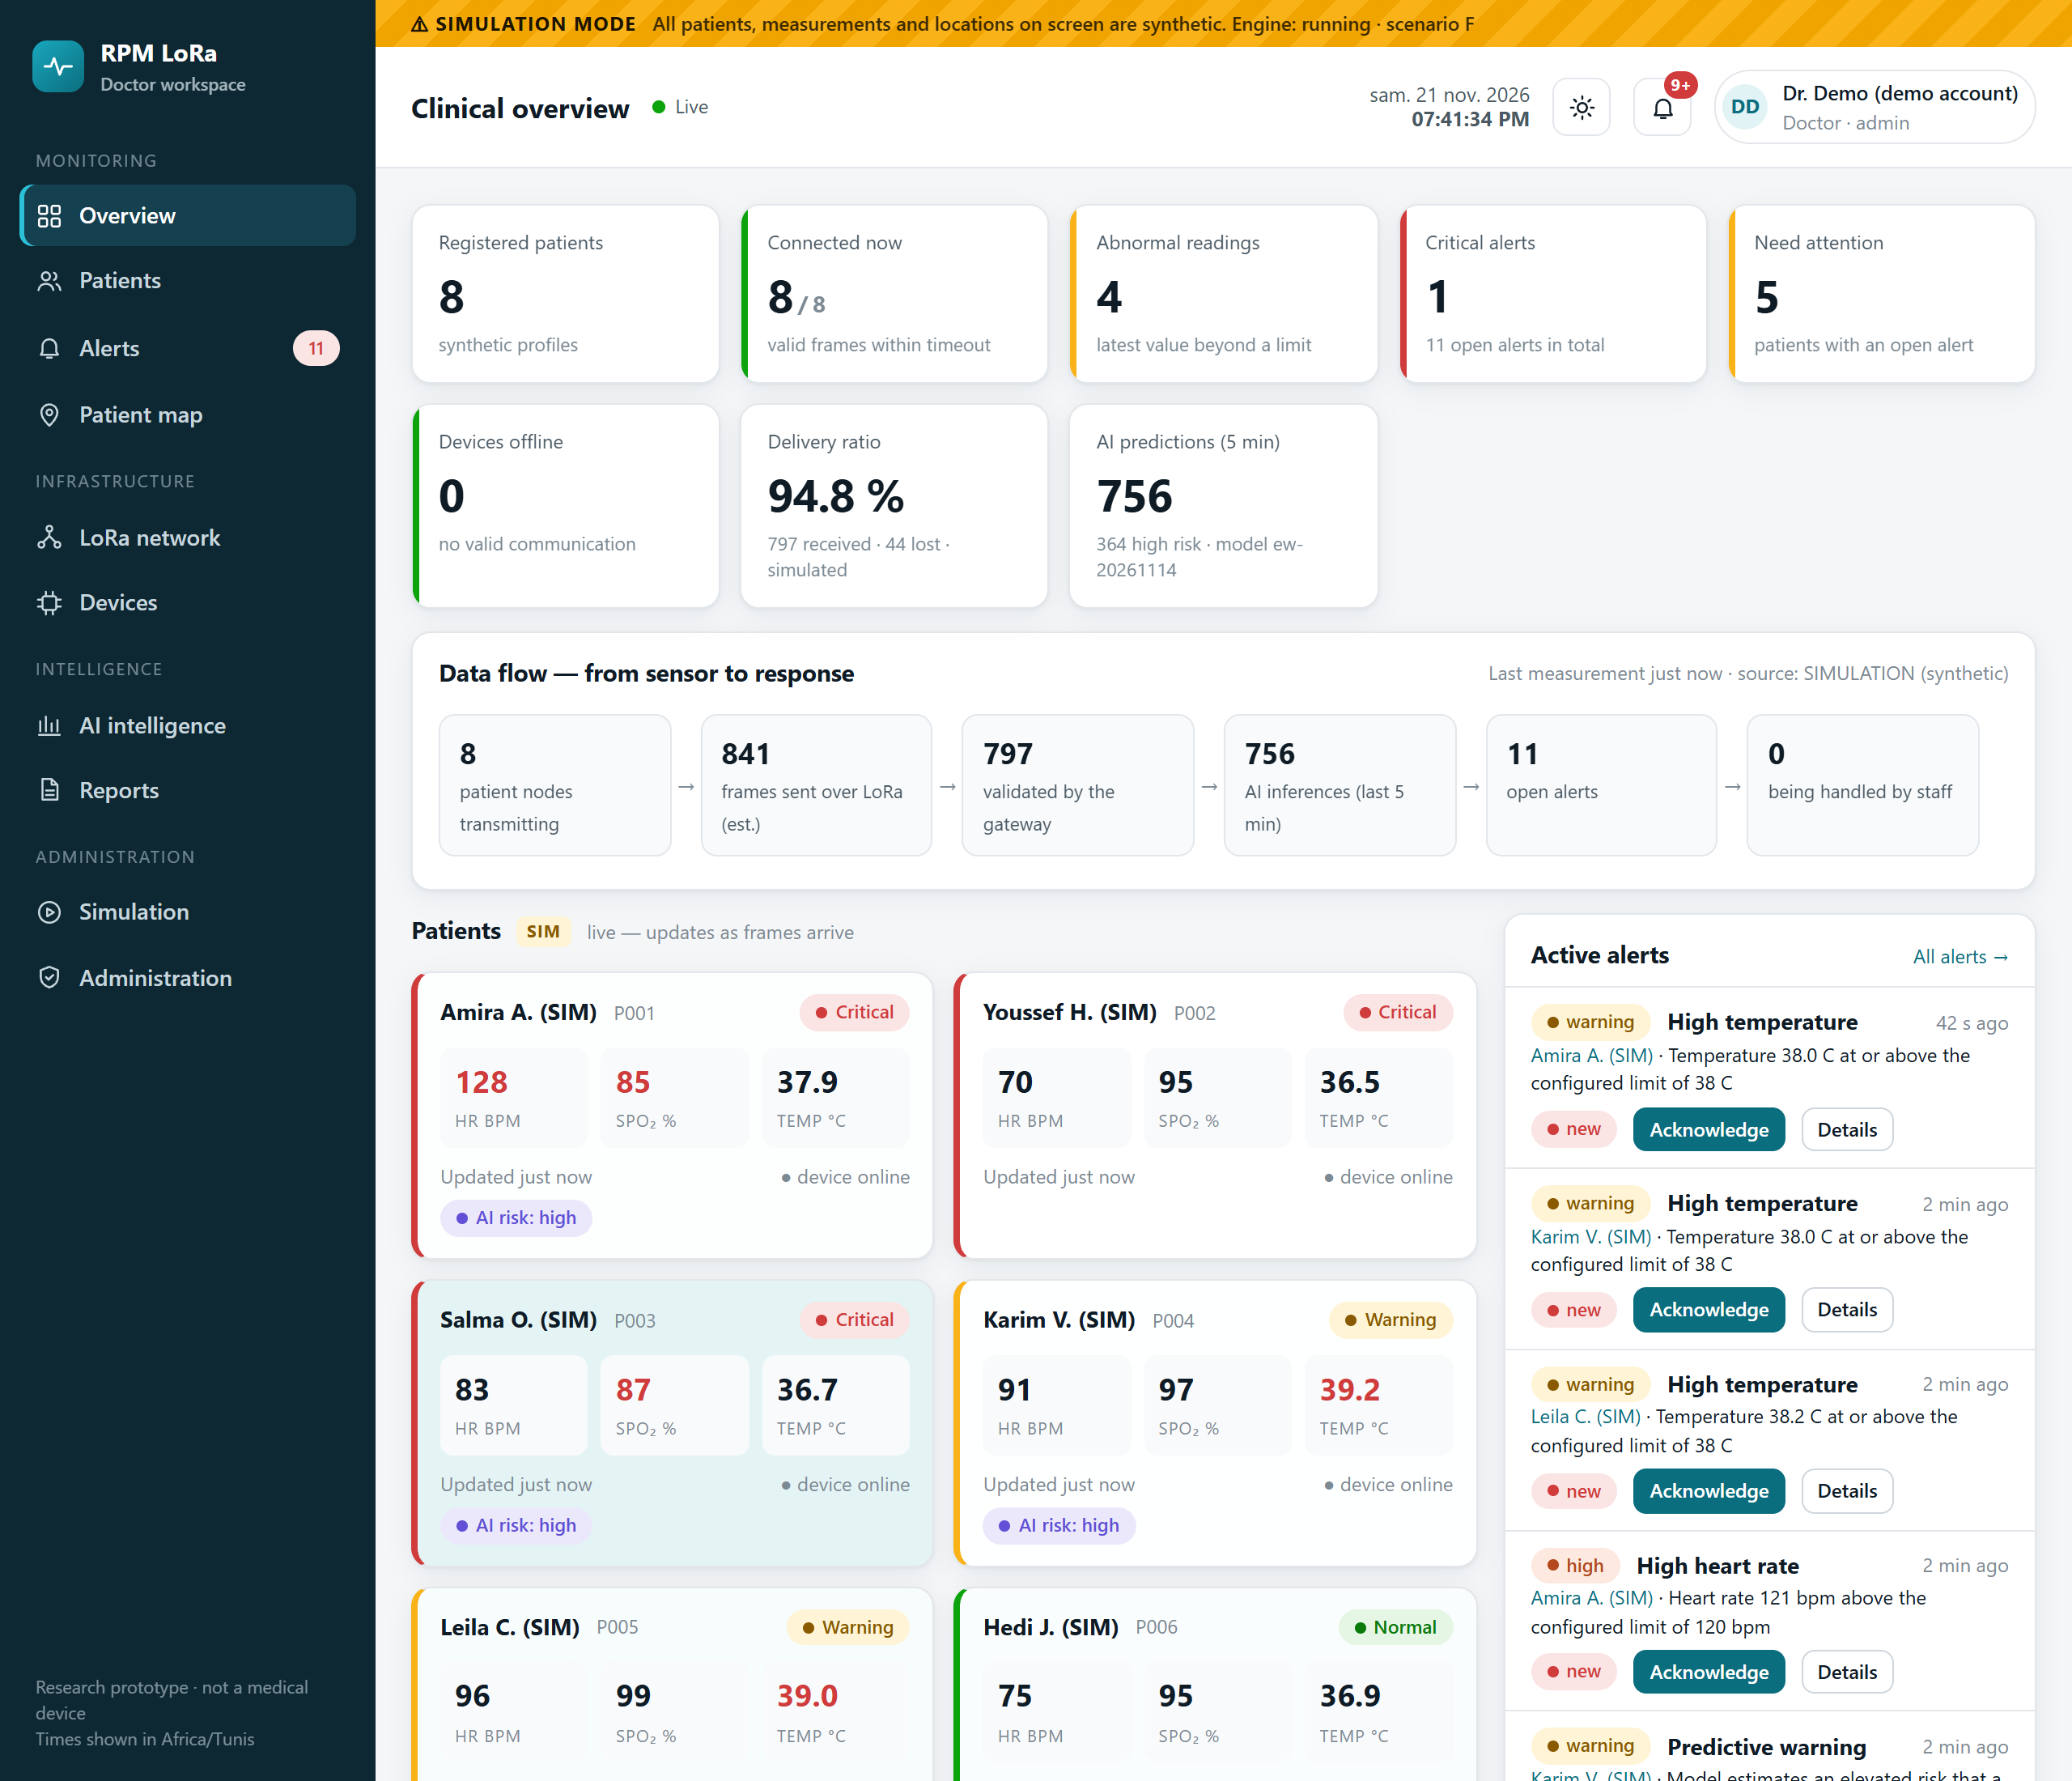
\includegraphics[height=5.7cm, trim=480 630 30 0, clip]{dashboard_overview.png}\label{fig:dash_overview}}\hfill
\subfloat[Patient view, scenario G: trends with alert limits (gaps are never interpolated); the predictive warning (07:46) precedes the heart-rate threshold alert (07:47).]{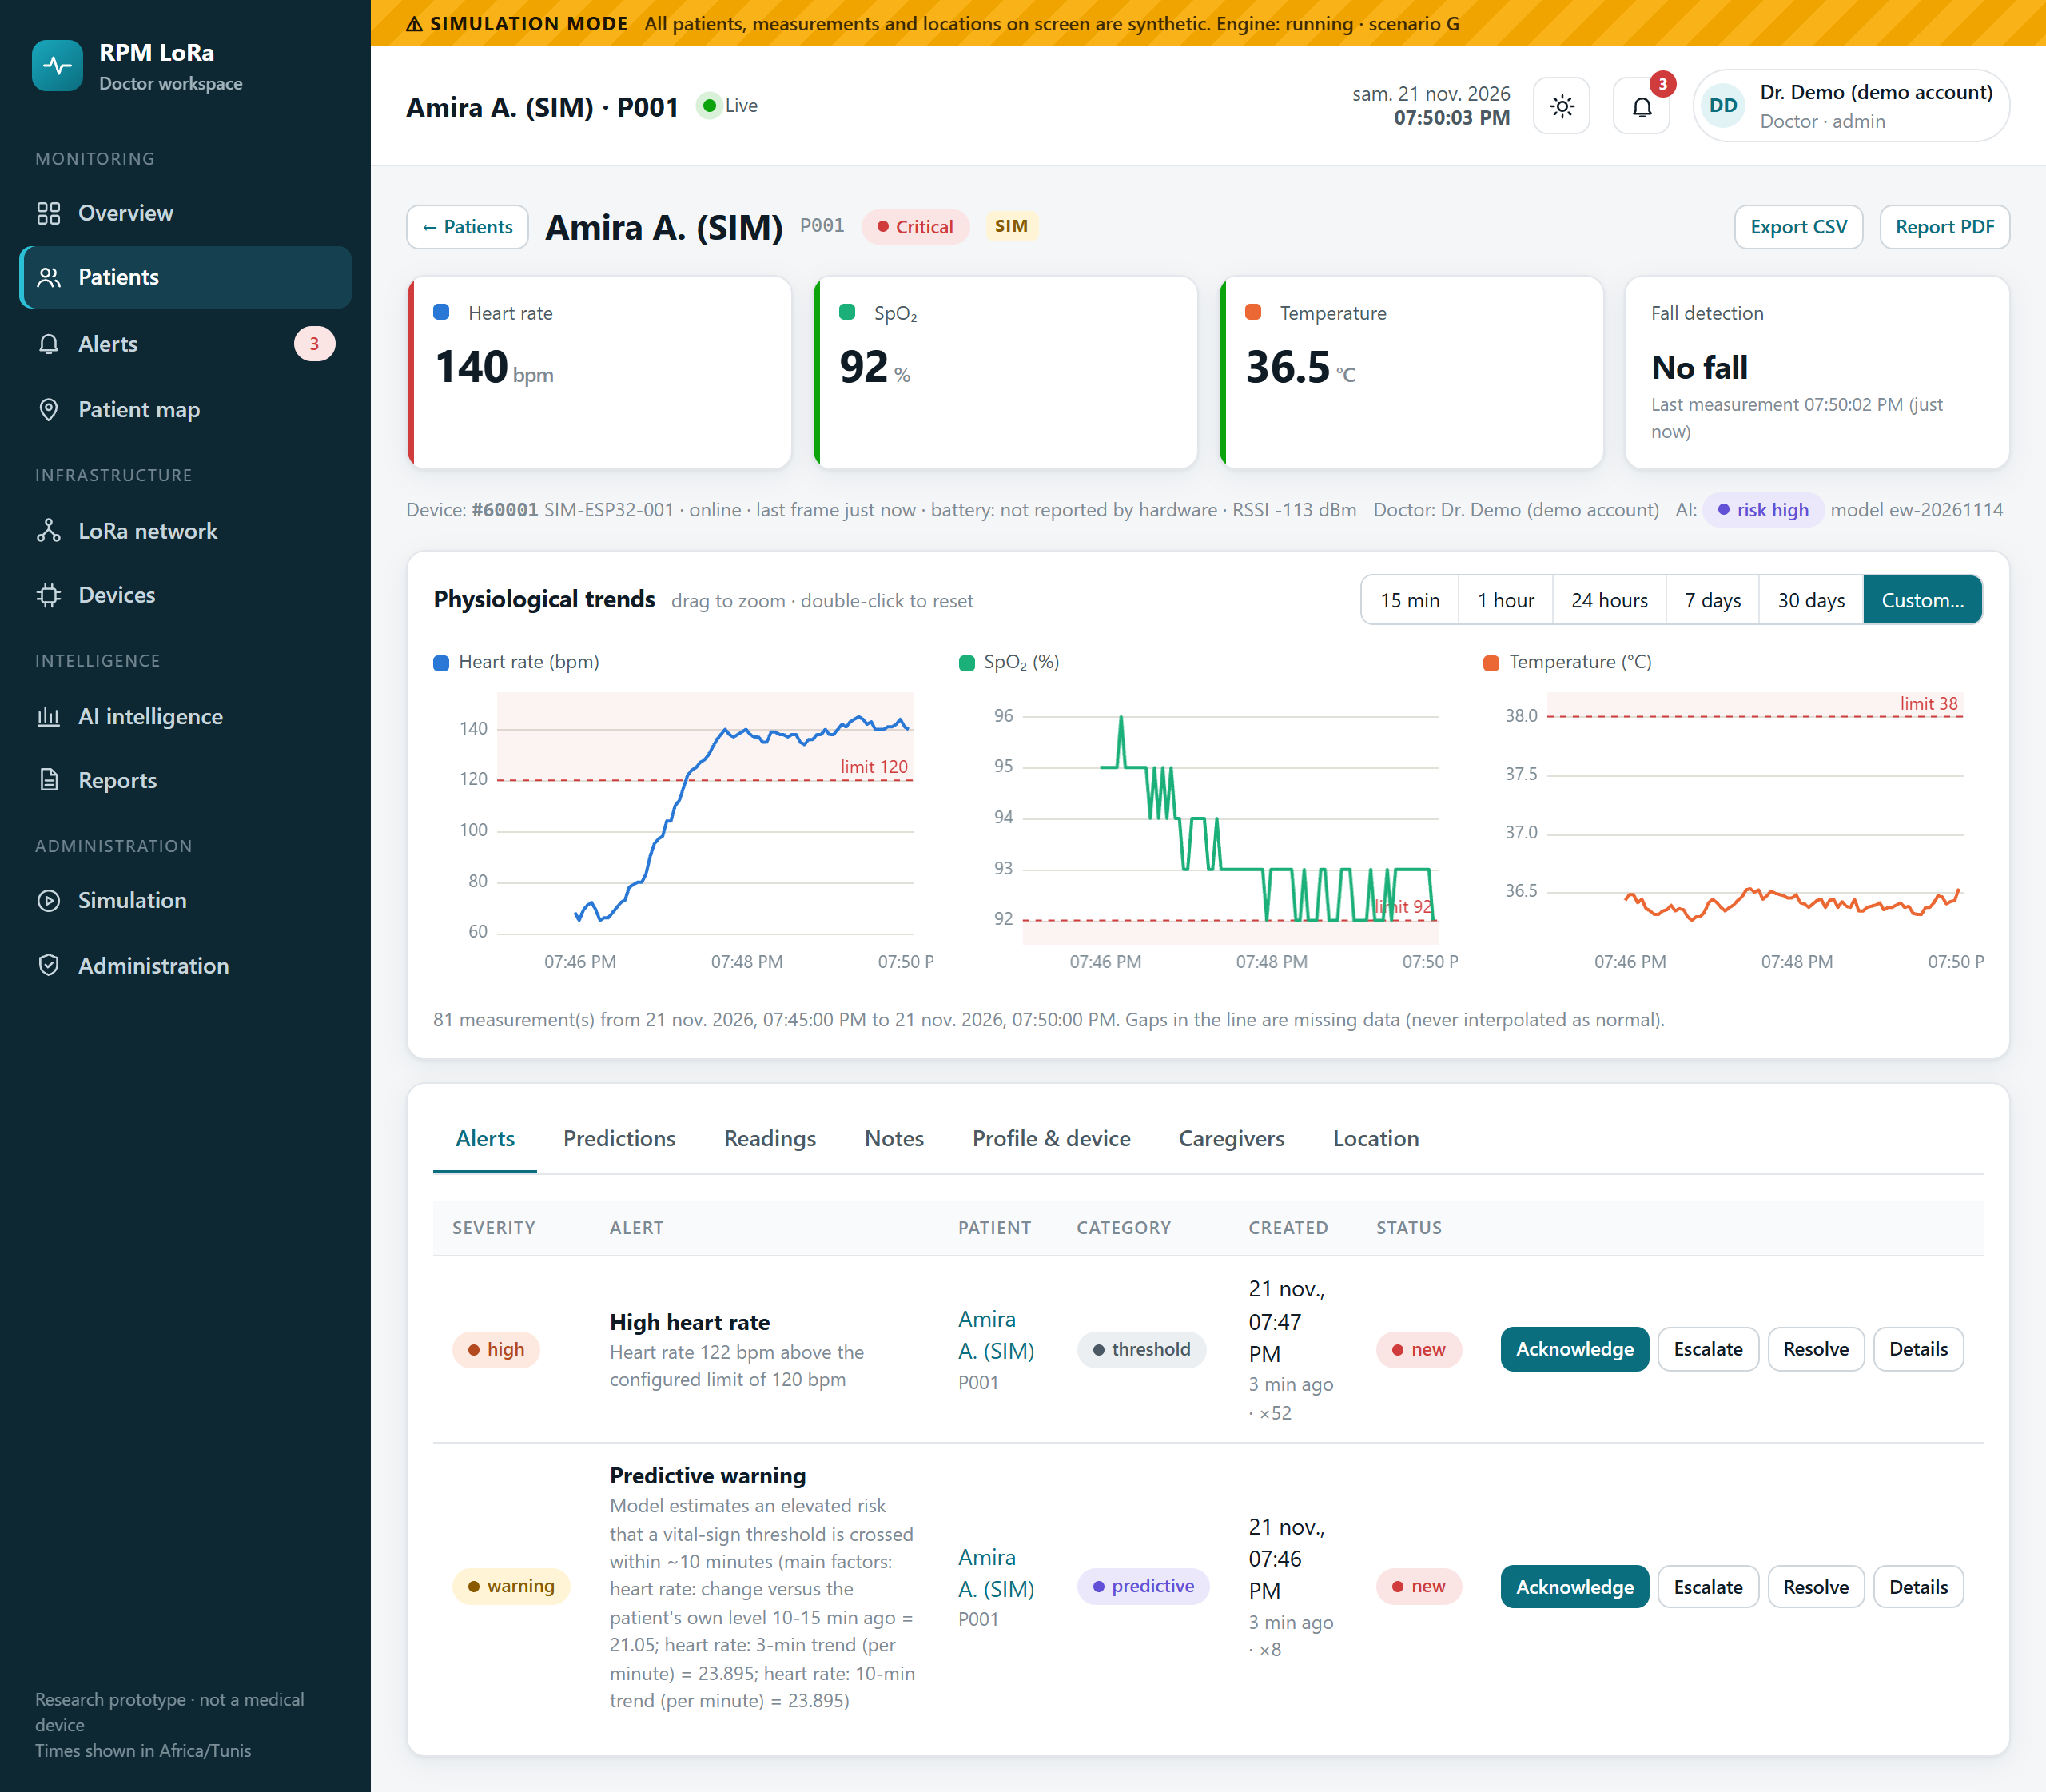
\includegraphics[height=5.7cm, trim=495 37 30 688, clip]{patient_monitoring.png}\label{fig:dash_patient}}
\caption{Real screenshots of the web dashboard in \emph{simulation mode}: all patients and values are synthetic, as stated by the banner and the ``(SIM)'' labels.}
\label{fig:dashboard}
\end{figure*}

The dashboard (Fig.~\ref{fig:dashboard}) is a build-free JavaScript application on the gateway's REST API. Server-side role-based access control yields three experiences: doctors see all patients, alerts, predictions, devices and reports; medical assistants see only assigned patients and acknowledge or escalate alerts; family caregivers see one patient in a simplified view, only after a consent record exists. The overview's data-flow strip (frames sent, validated, inferred, alerted, handled) makes radio losses visible to clinicians. The views keep four information layers apart: raw measurements (trend charts), threshold alerts, statistics (delivery ratio and RSSI/SNR per device on the network page) and model predictions with their main contributing features. Alerts follow a lifecycle (new, acknowledged, assigned, escalated, resolved or false positive) with automatic escalation when overdue. Fig.~\ref{fig:dash_patient} illustrates the workflow in simulation only; it is not evidence of clinical performance.

% =====================================================================================================================
\section{Data Analysis}
No real patient data were used. Model development relies on the synthetic dataset \texttt{synth-v2} (seed 20261114): 600 profiles of 8\,h sampled every 15, 30 or 60\,s (184/210/206 profiles), 627{,}099 samples, with baselines HR 58--92\,bpm, SpO$_2$ 94.5--98.8\,\% and temperature 36.2--37.1\,\textdegree C. Episodes model deterioration (HR rise 157, SpO$_2$ decline 152, combined 102, fever 94, abrupt 44, fall 29) and deliberately benign confounders (138 HR, 71 SpO$_2$), plus missing samples, outages, sensor faults and single-sample artifacts. HR and SpO$_2$ are missing in 0.15\,\% of rows; samples beyond the alert limits amount to 1.24\,\% (HR), 1.98\,\% (SpO$_2$) and 1.84\,\% (temperature). Fig.~\ref{fig:hist} shows that abnormal values occupy thin tails, so any detector faces strong class imbalance, and that single values near a limit carry little information on their own.

\begin{figure}[!t]
\centering
% Fig. - distributions of the SYNTHETIC dataset synth-v2 (627,099 samples, 600 profiles); red = beyond the alert limit.
% Data: figures/data/hist_{hr,spo2,temp}.dat (tools/make_figure_data.py). Zero bins are mapped below the axis (log scale).
\begin{tikzpicture}
\begin{groupplot}[
  group style={group size=3 by 1, horizontal sep=0.35cm, y descriptions at=edge left},
  width=0.355\linewidth, height=3.5cm, ymode=log, log origin=infty, ymin=1, ymax=4e5,
  ylabel={Samples}, ytick={1,1e2,1e4}, tick label style={font=\scriptsize}, label style={font=\small},
  xlabel style={yshift=2pt}, ylabel style={yshift=-3pt}, axis on top,
]
\nextgroupplot[xlabel={HR (bpm)}, xmin=40, xmax=200, xtick={60,120,180}]
\addplot[ybar interval, fill=swc!55, draw=swc!70, line width=.1pt] table[x=x, y expr=\thisrow{normal}+0.001] {figures/data/hist_hr.dat};
\addplot[ybar interval, fill=red!65, draw=red!75!black, line width=.1pt] table[x=x, y expr=\thisrow{beyond}+0.001] {figures/data/hist_hr.dat};
\draw[densely dashed, red!70!black] (axis cs:120,1) -- (axis cs:120,4e5);
\nextgroupplot[xlabel={SpO$_2$ (\%)}, xmin=70, xmax=101, xtick={75,85,92,100}]
\addplot[ybar interval, fill=swc!55, draw=swc!70, line width=.1pt] table[x=x, y expr=\thisrow{normal}+0.001] {figures/data/hist_spo2.dat};
\addplot[ybar interval, fill=red!65, draw=red!75!black, line width=.1pt] table[x=x, y expr=\thisrow{beyond}+0.001] {figures/data/hist_spo2.dat};
\draw[densely dashed, red!70!black] (axis cs:92,1) -- (axis cs:92,4e5);
\nextgroupplot[xlabel={Temperature (\textdegree C)}, xmin=35, xmax=41, xtick={36,38,40}]
\addplot[ybar interval, fill=swc!55, draw=swc!70, line width=.1pt] table[x=x, y expr=\thisrow{normal}+0.001] {figures/data/hist_temp.dat};
\addplot[ybar interval, fill=red!65, draw=red!75!black, line width=.1pt] table[x=x, y expr=\thisrow{beyond}+0.001] {figures/data/hist_temp.dat};
\draw[densely dashed, red!70!black] (axis cs:38,1) -- (axis cs:38,4e5);
\end{groupplot}
\end{tikzpicture}

\caption{Distributions of the synthetic dataset (log scale); red bins lie beyond the alert limit (dashed). Synthetic values, not clinical observations.}
\label{fig:hist}
\end{figure}

% =====================================================================================================================
\section{Predictive Model}
\subsection{Task, features and selection}
The model estimates whether a \emph{sustained} threshold condition (HR $>$\,120\,bpm, SpO$_2$ $<$\,92\,\% or temperature $\geq$\,38.0\,\textdegree C on two consecutive samples) starts within the next 10\,min, given the last 15\,min. Requiring two consecutive samples prevents single-sample artifacts from becoming labels. Per sample, 38 features are computed: level, spread, extremes, 3- and 10-min slopes, change versus the patient's own baseline 10--15\,min earlier, median of the last three samples, missing fraction, distance to each limit and extrapolated time to reach it, sampling gap and recent fall. Data are split by patient (60/20/20\,\%: 360/120/120 profiles; 349{,}341/120{,}212/116{,}861 rows). Logistic regression, random forest and histogram gradient boosting (HGB)~\cite{pedregosa2011sklearn,ke2017lightgbm} were compared with an isolation forest~\cite{liu2008iforest} and a trend-extrapolation rule. The rule ``highest validation PR-AUC among deployable models; within 0.01, lowest latency'' selected HGB: it ties the random forest on test PR-AUC (Table~\ref{tab:models}) but is about ten times faster. The high-risk threshold (0.645) maximizes F2 on validation, weighting recall above precision as missed deteriorations are costlier than false alarms; a medium level (0.231) guarantees validation recall $\geq$\,0.80. Isotonic calibration~\cite{zadrozny2002calibration} gives an expected calibration error of 0.0008, and each prediction lists its main contributing features by occlusion.

\begin{table}[!t]
\caption{Held-out synthetic test set (116{,}861 rows, 1.55\,\% positive); thresholds frozen on validation}
\label{tab:models}
\centering\footnotesize
\setlength{\tabcolsep}{2.6pt}
\begin{tabular}{@{}lccccccc@{}}
\toprule
Model & PR-AUC & ROC & Prec. & Rec. & F1 & Episodes & FA/day\\
\midrule
\textbf{HGB (deployed)} & \textbf{0.543} & 0.886 & \textbf{0.433} & 0.666 & \textbf{0.525} & 92/97 & \textbf{7.06}\\
Random forest & 0.543 & 0.897 & 0.420 & 0.689 & 0.522 & 92/97 & 7.06\\
Logistic regr. & 0.413 & 0.892 & 0.307 & 0.604 & 0.407 & 91/97 & 10.49\\
Isolation forest$^\dagger$ & 0.259 & 0.858 & 0.277 & 0.599 & 0.379 & 92/97 & 8.89\\
Trend rule$^\dagger$ & 0.372 & 0.877 & 0.241 & 0.595 & 0.343 & 94/97 & 21.58\\
\bottomrule
\multicolumn{8}{@{}L{\linewidth}@{}}{\scriptsize $^\dagger$Baselines, not deployable. Episodes: threshold-crossing episodes warned in advance. FA/day: false-alarm episodes per patient-day.}
\end{tabular}
\end{table}

\subsection{Evaluation}
With 1.55\,\% positives, accuracy (0.981) is dominated by the negative class and is not informative; PR curves are preferred~\cite{saito2015pr}. At the operating point (Fig.~\ref{fig:curves}) the model has recall 0.666, precision 0.433 and specificity 0.986 (1210 true and 1582 false positives, 606 false negatives). Episode-level metrics matter more for alerting: 92 of 97 test episodes were flagged in advance, with a median lead time of 8.5\,min (25th percentile 6.0\,min), at the price of 7.06 false-alarm episodes per patient-day, which is too high for unattended use and calls for alert aggregation and clinician-tuned thresholds. Fig.~\ref{fig:traj} shows one profile chosen by a fixed rule: the score crosses the high-risk level 3.5\,min before the sustained breach, while two isolated heart-rate artifacts ($-31$ and $-8$\,min) produce transient spikes, a typical source of false alarms.

\begin{figure}[!t]
\centering
% Fig. - held-out SYNTHETIC test set (116,861 rows, 1.55 % positive): PR and ROC curves of the deployed model ew-20261114.
% Curves: figures/data/{pr,roc}.dat (copied from ml/models/ew-20261114/curves.json). Operating point = frozen validation
% threshold 0.645 (metrics.json: precision 0.4334, recall 0.6663, FPR 0.0138).
\begin{tikzpicture}
\begin{groupplot}[
  group style={group size=2 by 1, horizontal sep=0.95cm},
  width=0.565\linewidth, height=0.5\linewidth, xmin=0, xmax=1, ymin=0, ymax=1.02,
  xtick={0,0.5,1}, ytick={0,0.5,1}, tick label style={font=\tiny}, label style={font=\scriptsize},
  title style={font=\scriptsize, yshift=-4pt}, xlabel style={yshift=3pt}, ylabel style={yshift=-4pt}, grid=major, grid style={black!10},
]
\nextgroupplot[xlabel={Recall}, ylabel={Precision}, title={PR curve, AUC 0.543}]
\addplot[swc, line width=.8pt] table[x=recall, y=precision] {figures/data/pr.dat};
\addplot[black!50, densely dashed] coordinates {(0,0.01554) (1,0.01554)};
\addplot[only marks, mark=*, mark size=1.6pt, red!80!black] coordinates {(0.6663,0.4334)};
\node[font=\tiny, anchor=south west, align=left] at (axis cs:0.02,0.03) {prevalence 0.016};
\nextgroupplot[xlabel={False-positive rate}, ylabel={True-positive rate}, title={ROC curve, AUC 0.886}]
\addplot[swc, line width=.8pt] table[x=fpr, y=tpr] {figures/data/roc.dat};
\addplot[black!50, densely dashed] coordinates {(0,0) (1,1)};
\addplot[only marks, mark=*, mark size=1.6pt, red!80!black] coordinates {(0.01375,0.6663)};
\end{groupplot}
\end{tikzpicture}

\caption{PR and ROC curves of the deployed HGB model on the synthetic test set; red dot: frozen operating point (threshold 0.645); dashed: chance level.}
\label{fig:curves}
\end{figure}

\begin{figure}[!t]
\centering
% Fig. - one SYNTHETIC test-split profile (id 265, 30-s sampling, single SpO2-decline episode; selected by a fixed rule:
% lowest-id test profile with exactly one such episode starting after the first hour). Score = deployed model, recomputed
% sample by sample with gateway/inference.py (tools/make_figure_data.py -> figures/data/example_patient.dat).
\begin{tikzpicture}
\begin{groupplot}[
  group style={group size=1 by 3, vertical sep=0.12cm, x descriptions at=edge bottom},
  width=\linewidth, height=2.35cm, xmin=-40, xmax=15, unbounded coords=jump,
  tick label style={font=\tiny}, label style={font=\scriptsize}, ylabel style={align=center, yshift=-2pt},
  extra x ticks={0,7.283}, extra x tick labels={}, extra x tick style={grid=major, major grid style={black!45, densely dashed}},
  scale only axis=false,
]
\nextgroupplot[ylabel={HR\\[-2pt](bpm)}, ymin=60, ymax=132, ytick={80,120}]
\addplot[swc, line width=.55pt] table[x=tmin, y=hr] {figures/data/example_patient.dat};
\draw[red!70!black, densely dotted, line width=.6pt] (axis cs:-40,120) -- (axis cs:15,120);
\nextgroupplot[ylabel={SpO$_2$\\[-2pt](\%)}, ymin=87, ymax=101, ytick={90,95,100}]
\addplot[comc, line width=.55pt] table[x=tmin, y=spo2] {figures/data/example_patient.dat};
\draw[red!70!black, densely dotted, line width=.6pt] (axis cs:-40,92) -- (axis cs:15,92);
\nextgroupplot[ylabel={risk\\[-2pt]score}, ymin=0, ymax=1.05, ytick={0,0.5,1}, xlabel={Time relative to simulated episode onset (min)}, xtick={-40,-30,-20,-10,0,10}]
\addplot[hwc, line width=.6pt] table[x=tmin, y=score] {figures/data/example_patient.dat};
\draw[black!60, densely dotted] (axis cs:-40,0.231) -- (axis cs:15,0.231);
\draw[black!80, dashed] (axis cs:-40,0.645) -- (axis cs:15,0.645);
\node[font=\tiny, anchor=south west, inner sep=1pt] at (axis cs:-39.5,0.645) {high};
\node[font=\tiny, anchor=south west, inner sep=1pt] at (axis cs:-39.5,0.231) {medium};
\end{groupplot}
\end{tikzpicture}

\caption{Synthetic test profile 265 (SpO$_2$-decline episode, 30-s sampling). Vertical dashed lines: simulated episode onset (0\,min) and sustained-breach onset (+7.3\,min); dotted horizontal lines: alert limits. Bottom: model score recomputed sample by sample with the gateway inference code.}
\label{fig:traj}
\end{figure}

\subsection{Computational efficiency and clinical interpretation}
The HGB artifact is 450\,KiB. On the x86-64 development PC one prediction, including the 38 occlusion evaluations for the explanation, takes 6.1\,ms median (95th percentile 23.6\,ms); 20 patients at one sample per 30\,s need fewer than one prediction per second, so even a several-fold slower Raspberry~Pi~5 would remain far from saturation (an estimate; Pi~5 latency has not been measured). Deeper models are not justified by the 38 tabular features and the observed tie between ensembles. Clinically, the output is a decision-support score next to raw values and deterministic threshold alerts, not a diagnosis; it is not a validated score such as NEWS2~\cite{rcp2017news2}, and synthetic performance does not transfer to real patients without prospective evaluation.

% =====================================================================================================================
\section{Security and Data Protection}
Table~\ref{tab:security} separates implemented and tested mechanisms from gaps. Authenticity, integrity and replay protection of radio frames are implemented, but \emph{confidentiality} over the air is not: vital signs are sent in clear and can be observed by any receiver tuned to the channel. The recommended extension is AES-CCM or AES-GCM~\cite{nist80038d} payload encryption with per-device keys and a nonce derived from the persisted seqNo, which would add no bytes beyond the existing tag if the MAC is reused.

\begin{table}[!t]
\caption{Security mechanisms and verification status}
\label{tab:security}
\centering\footnotesize
\begin{tabularx}{\linewidth}{@{}L{1.7cm}YL{1.05cm}@{}}
\toprule
Aspect & Implementation & Status\\
\midrule
Frame integrity & HMAC-SHA256, 64-bit tag, per-device key; CRC-16; relays may change only hopCount & tested \ok\\
Replay & persisted 32-bit seqNo, 62-frame window per device & tested \ok\\
Confidentiality (radio) & none: payload in clear; AES-CCM/GCM proposed & gap\\
Keys at rest & device keys, TOTP secrets wrapped with AES-256-GCM & tested \ok\\
User login & scrypt hashes, lockout (5 failures, 30--900\,s), rate limit, optional TOTP & tested \ok\\
Sessions & HttpOnly SameSite=Strict cookie, 30\,min idle / 12\,h absolute, CSRF token & tested \ok\\
Authorization & server-side RBAC (3 roles), per-patient scope, consent for caregivers & tested \ok\\
Accountability & SHA-256 hash-chained audit log & tested \ok\\
Transport & HTTP only; TLS reverse proxy required for deployment & \pend\\
UART hop & unauthenticated serial line; HMAC end-to-end if raw frames are forwarded & \pend\\
\bottomrule
\end{tabularx}
\end{table}

% =====================================================================================================================
\section{Evaluation Summary and Engineering Challenges}
Table~\ref{tab:evidence} summarizes the evidence by category; no figure combines categories. Table~\ref{tab:challenges} lists the main problems met and how they were resolved.

\begin{table}[!t]
\caption{Evidence summary by category}
\label{tab:evidence}
\centering\footnotesize
\begin{tabularx}{\linewidth}{@{}L{1.35cm}Y@{}}
\toprule
Category & Result (source)\\
\midrule
Software test & 233/233 automated tests pass in 337\,s (pytest, 2026-11-21); C++ frame encoder byte-identical to Python reference\\
Physical & bench LoRa link operating, Heltec~V3 counting received packets (Fig.~\ref{fig:hardware_real}); UART to Pi configured, reception not confirmed\\
Simulation & PDR 79/80 = 98.75\,\%; 0 collisions, 0 duplicates; delay 78.08\,ms direct, +61.70\,ms per hop (OMNeT++ run r6)\\
Analytical & $T_{\mathrm{oa}}$ = 77.1\,ms for 34\,B; duty cycle 0.26\,\%; ALOHA success 0.90 for 20 nodes (Eq.~\ref{eq:toa})\\
Model eval. & PR-AUC 0.543, recall 0.666 at precision 0.433; 92/97 episodes, median lead 8.5\,min; 7.06 false-alarm episodes/patient-day (synthetic)\\
Software meas. & 6.1\,ms median inference with explanation on x86-64; 450\,KiB model; Pi~5 \pend\\
\bottomrule
\end{tabularx}
\end{table}

\begin{table}[!t]
\caption{Engineering challenges: root cause $\to$ solution}
\label{tab:challenges}
\centering\footnotesize
\begin{tabularx}{\linewidth}{@{}L{1.55cm}YL{1.15cm}@{}}
\toprule
Challenge & Root cause $\to$ solution & Status\\
\midrule
Pi~5: no data on \texttt{serial0} & alias pointed to the \texttt{ttyAMA10} debug UART, UART0 not on GPIO14/15 $\to$ \texttt{dtoverlay=uart0-pi5}, read \texttt{/dev/ttyAMA0}; check pins with \texttt{pinctrl} before suspecting hardware & fixed; RX \pend\\
Heltec~V3 TX pin & GPIO43 is UART0 TX of the CP2102 USB bridge $\to$ UART1 on GPIO2 via the GPIO matrix, RX disabled & applied; \pend\\
FLoRa for multi-hop RPM & gateway MAC does not drain a relay's queue; transmit power not initialised; airtime from a fixed 20/15-B payload $\to$ custom relay MAC and radio module (FLoRa unmodified); analytical $T_{\mathrm{oa}}$ reported (Fig.~\ref{fig:delay}) & done (sim.)\\
Artifact-driven labels & single-sample spikes labelled as events $\to$ sustained-breach target, median-of-three features & done\\
Simulated vs.\ physical data & shared identifiers and tables $\to$ separate database files, virtual IDs $\geq$\,60001, banner on every page & tested \ok\\
Pages jumping to the overview & concurrent navigation at sign-in left a hidden view refreshing $\to$ navigation counter discards stale views & fixed\\
\bottomrule
\end{tabularx}
\end{table}

% =====================================================================================================================
\section{Conclusion}
The prototype demonstrates a complete software path from an authenticated 34-byte LoRa frame to role-based clinical views and an on-gateway early-warning model, a bench LoRa link with a documented Raspberry~Pi~5 UART integration, and a multi-hop OMNeT++/FLoRa model with honest accounting of its airtime simplification. The decisive next steps are physical: assembling and flashing the physiological sensor node, validating the UART and SPI receive paths, measuring PDR, RSSI and delay on site, and measuring inference latency on the Pi~5. On the network side, the prepared FLoRa n1000 ADR/no-ADR/two-gateway configurations should be run with random traffic; on the security side, payload encryption and TLS are required before any deployment, and clinical use would additionally require real-patient data under ethical approval.

\bibliographystyle{IEEEtran}
\bibliography{references}

\end{document}
